\documentclass{article}

\usepackage{hyperref}                 % Hyperlinks
\hypersetup{
	hidelinks,                        % Hide link boxes
	colorlinks = true,
	citecolor = cyan,
	urlcolor = black,
	linkcolor = magenta
}
\usepackage{arxiv}
\usepackage{amsmath}
\usepackage[utf8]{inputenc} % allow utf-8 input
\usepackage[T1]{fontenc}    % use 8-bit T1 fonts
\usepackage{url}            % simple URL typesetting
\usepackage{booktabs}       % professional-quality tables
\usepackage{amsfonts}       % blackboard math symbols
\usepackage{amssymb}        % math symbols
\usepackage{nicefrac}       % compact symbols for 1/2, etc.
\usepackage{microtype}      % microtypography
\usepackage{cleveref}       % smart cross-referencing
\usepackage{graphicx}
\graphicspath{{../figures/}}
\usepackage{natbib}
\usepackage{xcolor}

\usepackage{subcaption}
\usepackage{threeparttable}

\title{Belief State Geometry in a Non-Ergodic Mess3 Transformer}

\renewcommand{\shorttitle}{Belief Geometry in Non-Ergodic Mess3}

\renewcommand{\headeright}{MATS Simplex takehome}
\renewcommand{\undertitle}{MATS Simplex takehome}

\date{March 2026}

\usepackage{authblk}
\renewcommand\Authfont{\bfseries}
\setlength{\affilsep}{0em}

\author{Tom Kimpson}

\begin{document}
\maketitle


\section{Introduction}

Transformers trained on next-token prediction learn internal representations of their input, but what structure do those representations take? \citet{shai2024} showed that for the Mess3 process, a simple hidden Markov model, a transformer's activations linearly encode the Bayesian belief states and form fractal geometry in the residual stream. That work studied a single ergodic process. Real language is non-ergodic: a stream of text might come from different modes (topics, genres), each with its own statistical regularities. Non-ergodicity introduces a second latent variable, the identity of the mode that generated the current sequence, which the model must infer from tokens while also tracking within-mode dynamics.

This mode-inference problem is a minimal model of in-context learning: just as a language model reading the opening sentences of a text must infer whether it is reading legal prose or casual dialogue and adjust its predictions accordingly, our transformer must identify which Mess3 component generated the current sequence from the token statistics alone. Studying how a small model solves this simpler problem may clarify how larger models handle variation in register and domain.

We extend the Mess3 setup to a non-ergodic mixture of three components with different parameters, where each training sequence is generated entirely by one component. The data-generating process has two latent factors: component identity (which Mess3 process) and hidden state (which of the 3 states within that process). This makes it a direct test of the factored representation hypothesis of \citet{shai2026}: does the transformer learn to represent these factors in orthogonal subspaces, or in a joint product space? Code is available at \url{https://github.com/tomkimpson/simplex-test}.\footnote{LLM declaration: the code used in this work was generated with the assistance of Claude Opus 4.6}


\section{Methods}

\subsection{The Mess3 Process}

The Mess3 process \citep{shai2024} is a 3-state, 3-token hidden Markov model parameterised by $(\alpha, x)$. Each token is informative about a specific hidden state: token $k$ appears more frequently when the process is in state $k$, with $\alpha$ controlling how informative tokens are (higher $\alpha$ means more informative). Bayesian belief updating produces posterior distributions over the 3 hidden states that live in a 2-simplex, and these belief states form fractal geometry whose structure is determined by $(\alpha, x)$. The entropy rate of each component is computed analytically from the closed-form emission matrix via $H = -\sum_s \pi(s) \sum_k E_{sk} \log_2 E_{sk}$, where $\pi$ is the uniform stationary distribution over the 3 hidden states.

\subsection{Non-Ergodic Dataset}

We construct a non-ergodic mixture of three Mess3 components with distinct parameters:

\begin{table}[h]
\centering
\caption{Mess3 component parameters.}
\label{tab:components}
\begin{tabular}{@{}lccll@{}}
\toprule
Component & $\alpha$ & $x$ & Entropy Rate (bits) & Character \\
\midrule
A & 0.90 & 0.05 & 0.876 & Sparse fractal, highly informative tokens \\
B & 0.70 & 0.10 & 1.387 & Medium fractal, moderate informativeness \\
C & 0.55 & 0.05 & 1.482 & Dense fractal, weakly informative tokens \\
\bottomrule
\end{tabular}
\end{table}

These parameters are chosen to produce well-separated entropy rates and visually distinct fractal geometries. Each training sequence of length 16 is generated entirely by one component, drawn uniformly; the component label is not provided to the model and must be inferred from the token statistics. The training set contains 300,000 sequences (100k per component) and the evaluation set 30,000. We train a small causal decoder-only transformer with 3 layers, $d_\text{model} = 64$, 4 attention heads, MLP hidden dimension 256, learned positional encodings, and pre-norm LayerNorm ($\sim$150k parameters total). Training uses Adam (lr $= 10^{-3}$), batch size 64, for 200 epochs on cross-entropy next-token prediction loss.


\section{Pre-Registered Geometric Predictions}

We write these predictions before examining any activations, following the honour code.

\subsection{Mathematical Derivation}

Bayesian updating on the Mess3 process produces belief states (posterior distributions over hidden states) that live in a 2-simplex and form fractal geometry determined by $(\alpha, x)$. \citet{shai2024} showed that for a single Mess3 component, a transformer's activations linearly encode this belief geometry. Our non-ergodic process has two latent factors, component identity and within-component hidden state, so the question is how the transformer organises both.

The joint latent space has $3 \times 3 = 9$ states, and the full belief over this space lives in an 8-simplex. A joint (unfactored) representation would track all 9 states simultaneously, requiring up to $(\prod_n d_n) - 1 = 8$ dimensions. A factored representation separately tracks a belief over 3 components and a belief over 3 hidden states, requiring only $\sum_n (d_n - 1) = (3-1) + (3-1) = 4$ dimensions \citep{shai2026}. The important asymmetry is that component identity is fixed per sequence and becomes increasingly identifiable from context, while the hidden state evolves dynamically. This asymmetry should push the model to separate the two factors. \citet{shai2026} show that transformers have an inductive bias towards such factored representations, placing each factor in orthogonal subspaces, and that this factoring persists even when it is lossy because it acts as a representational attractor.

However, since each component has distinct fractal geometry, a purely factored representation with a shared 2D hidden-state subspace may be insufficiently expressive. The model may instead learn separate 2D belief subspaces per component with orthogonal component offsets, yielding $\sim$6D effective dimensionality, intermediate between the factored (4D) and joint (8D) predictions.

\subsection{Geometric Intuition}

Our prediction for the geometry of the activations is as follows. The residual stream should contain three distinct clusters, one per component, arranged as vertices of a 2-simplex in a component-identity subspace. Within each cluster, the activations should trace out the fractal belief-simplex geometry characteristic of that component's parameters: a sparse, edge-concentrated pattern for component A (high $\alpha$), a Sierpinski-like triangular structure for B (moderate $\alpha$), and a dense filled cloud for C (low $\alpha$). The component-identity directions and the within-component belief directions should be approximately orthogonal, so that the full geometry consists of three fractal 2-simplices embedded in $\sim$4--6 dimensions of the 64-dimensional residual stream.

\subsection{Alternative Geometries}

Three alternative geometries are worth considering. First, rather than orthogonal subspaces, the model might learn a single shared 2D belief subspace with component identity encoded as affine offsets: three translated copies of the same fractal, rather than three fractals in orthogonal subspaces. Second, the model might track the full joint belief over all 9 states without factoring, producing a higher-dimensional ($\sim$8D) representation with weaker component clustering. Third, the model might find a compressed encoding exploiting approximate symmetries between the three fractal geometries, using fewer dimensions than any of these predictions.

\subsection{Context Position and Layer Dependence}

This geometry should emerge progressively along both axes. In context position, early tokens (positions 0--2) provide insufficient statistical evidence to distinguish components, so the three clusters should overlap with near-uniform within-component beliefs. Over middle positions (3--8) the components' distinct entropy rates and transition statistics become identifiable, and we predict a sharp transition to near-perfect component separation with visible fractal structure at late positions (9--15). Across layers, the embedding layer should encode only token identity with no component information, layers 0--1 should begin aggregating token statistics for both component identification and belief tracking, and layer 2 should show the clearest component separation and sharpest fractal geometry, with peak $R^2$ from linear regression to oracle beliefs.


\section{Results}

The model converges after 200 epochs, with per-component losses approaching but not reaching the theoretical entropy rates (residual gaps of 0.088--0.142 nats, where cross-entropy loss is measured in nats and entropy rates from \Cref{tab:components} (in bits) are converted via $H_\text{nats} = H_\text{bits} \times \ln 2$). We examine the residual stream geometry with three tools: PCA to visualize the activation manifold, linear regression to quantify belief encoding, and probing to measure component identification.

\subsection{PCA of Residual Stream}

\begin{figure}[ht]
    \centering
    \begin{subfigure}[b]{\textwidth}
        \centering
        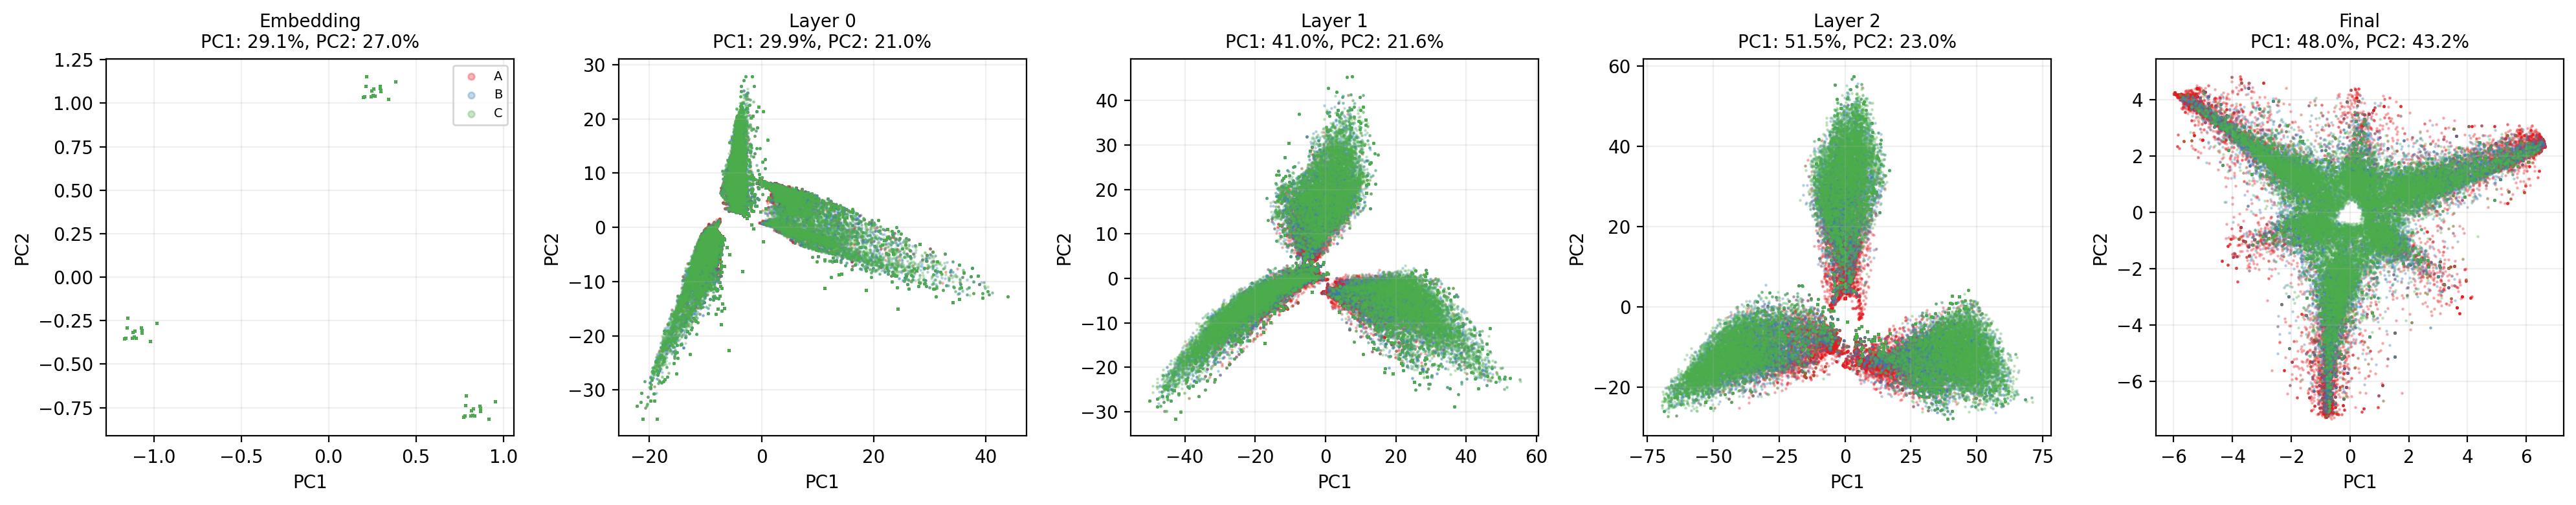
\includegraphics[width=\textwidth]{pca_by_layer.png}
        \caption{Across layers. The dominant structure is a three-armed pattern corresponding to token identity, not component identity. Components A, B, C (colored) largely overlap within this structure.}
        \label{fig:pca_layer}
    \end{subfigure}
    \vspace{1em}
    \begin{subfigure}[b]{\textwidth}
        \centering
        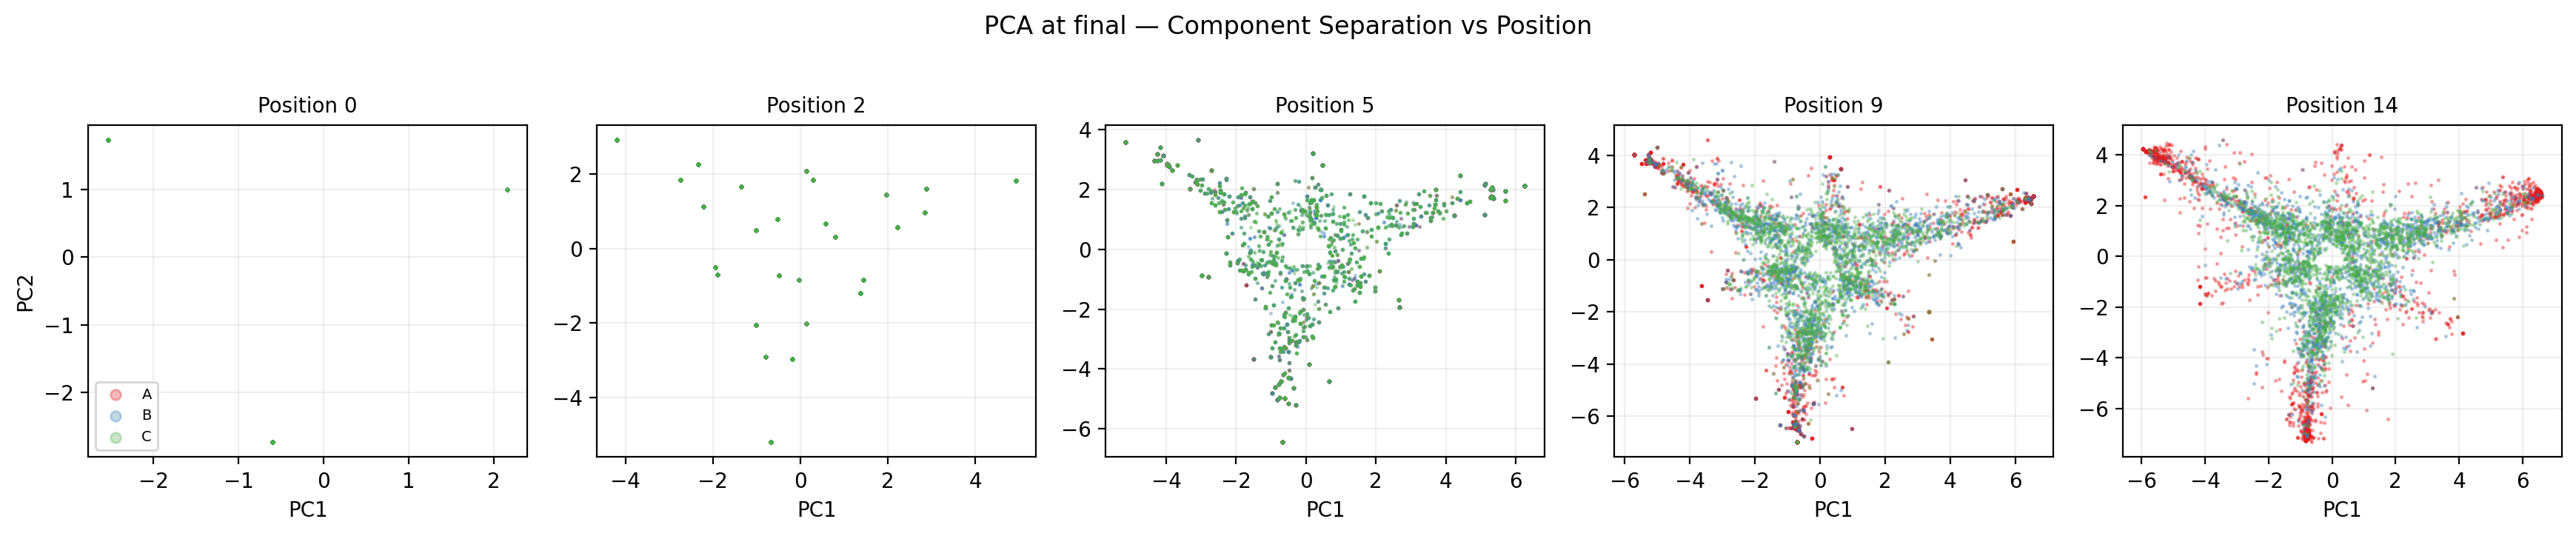
\includegraphics[width=\textwidth]{pca_by_position.png}
        \caption{Across context positions at the final layer. The three-armed token structure emerges with increasing context, but component separation remains partial even at late positions.}
        \label{fig:pca_position}
    \end{subfigure}
    \vspace{1em}
    \begin{subfigure}[b]{\textwidth}
        \centering
        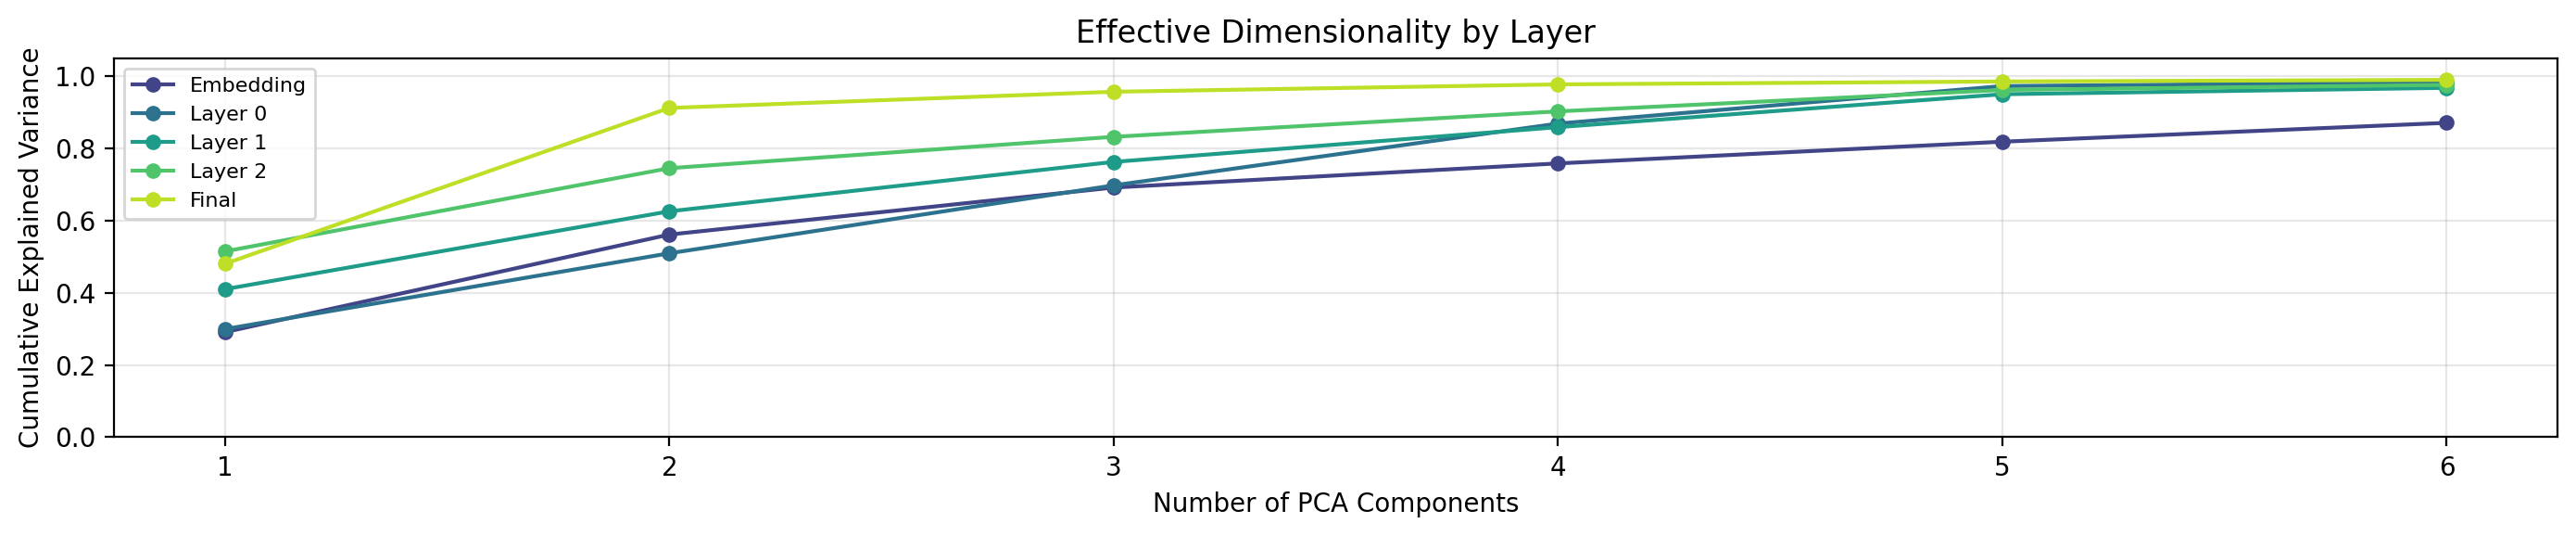
\includegraphics[width=\textwidth]{explained_variance.png}
        \caption{Cumulative explained variance by number of PCA components across layers. The final layer concentrates into $\sim$2 effective dimensions, while earlier layers retain higher dimensionality.}
        \label{fig:explained_variance}
    \end{subfigure}
    \caption{PCA of residual stream activations.}
    \label{fig:pca}
\end{figure}

PCA of the residual stream (\Cref{fig:pca_layer}) shows that the dominant structure across layers is a three-armed pattern corresponding to the three token types, not component separation. At the embedding layer, three tight clusters appear (one per token) with all components overlapping within each. Through layers 0--2, these clusters elongate into a three-armed radial structure with increasing internal complexity along each arm, but components A, B, and C remain largely overlapping throughout. At the final post-LayerNorm representation, the first two principal components explain 48\% and 43\% of the variance, and the structure compresses into a more compact form with some visible component offset but no clean separation.

Examining the final layer across context positions (\Cref{fig:pca_position}) shows a similar picture. At position 0, only the three token clusters are visible. The three-armed structure emerges by position 5 and grows more elaborate at later positions, but component separation remains partial even at position 14. Components are interleaved within the token-dominated structure rather than forming distinct clusters.

This contrasts with our prediction of three clearly separated component clusters. The PCA projection is dominated by token identity, which accounts for most of the variance, while component information appears to be encoded in directions that the first two principal components do not capture. The effective dimensionality analysis (\Cref{fig:explained_variance}) supports this interpretation: the final layer compresses to $\sim$2D (matching the 3-token output simplex), while earlier layers retain higher effective dimensionality (the first 2 PCs capture only $\sim$50--55\% of variance at the embedding and layer 0, vs.\ $\sim$91\% at the final layer). Component and belief information may well be present in these additional dimensions but invisible in a 2D PCA projection.

\subsection{Belief Regression}

\begin{figure}[ht]
    \centering
    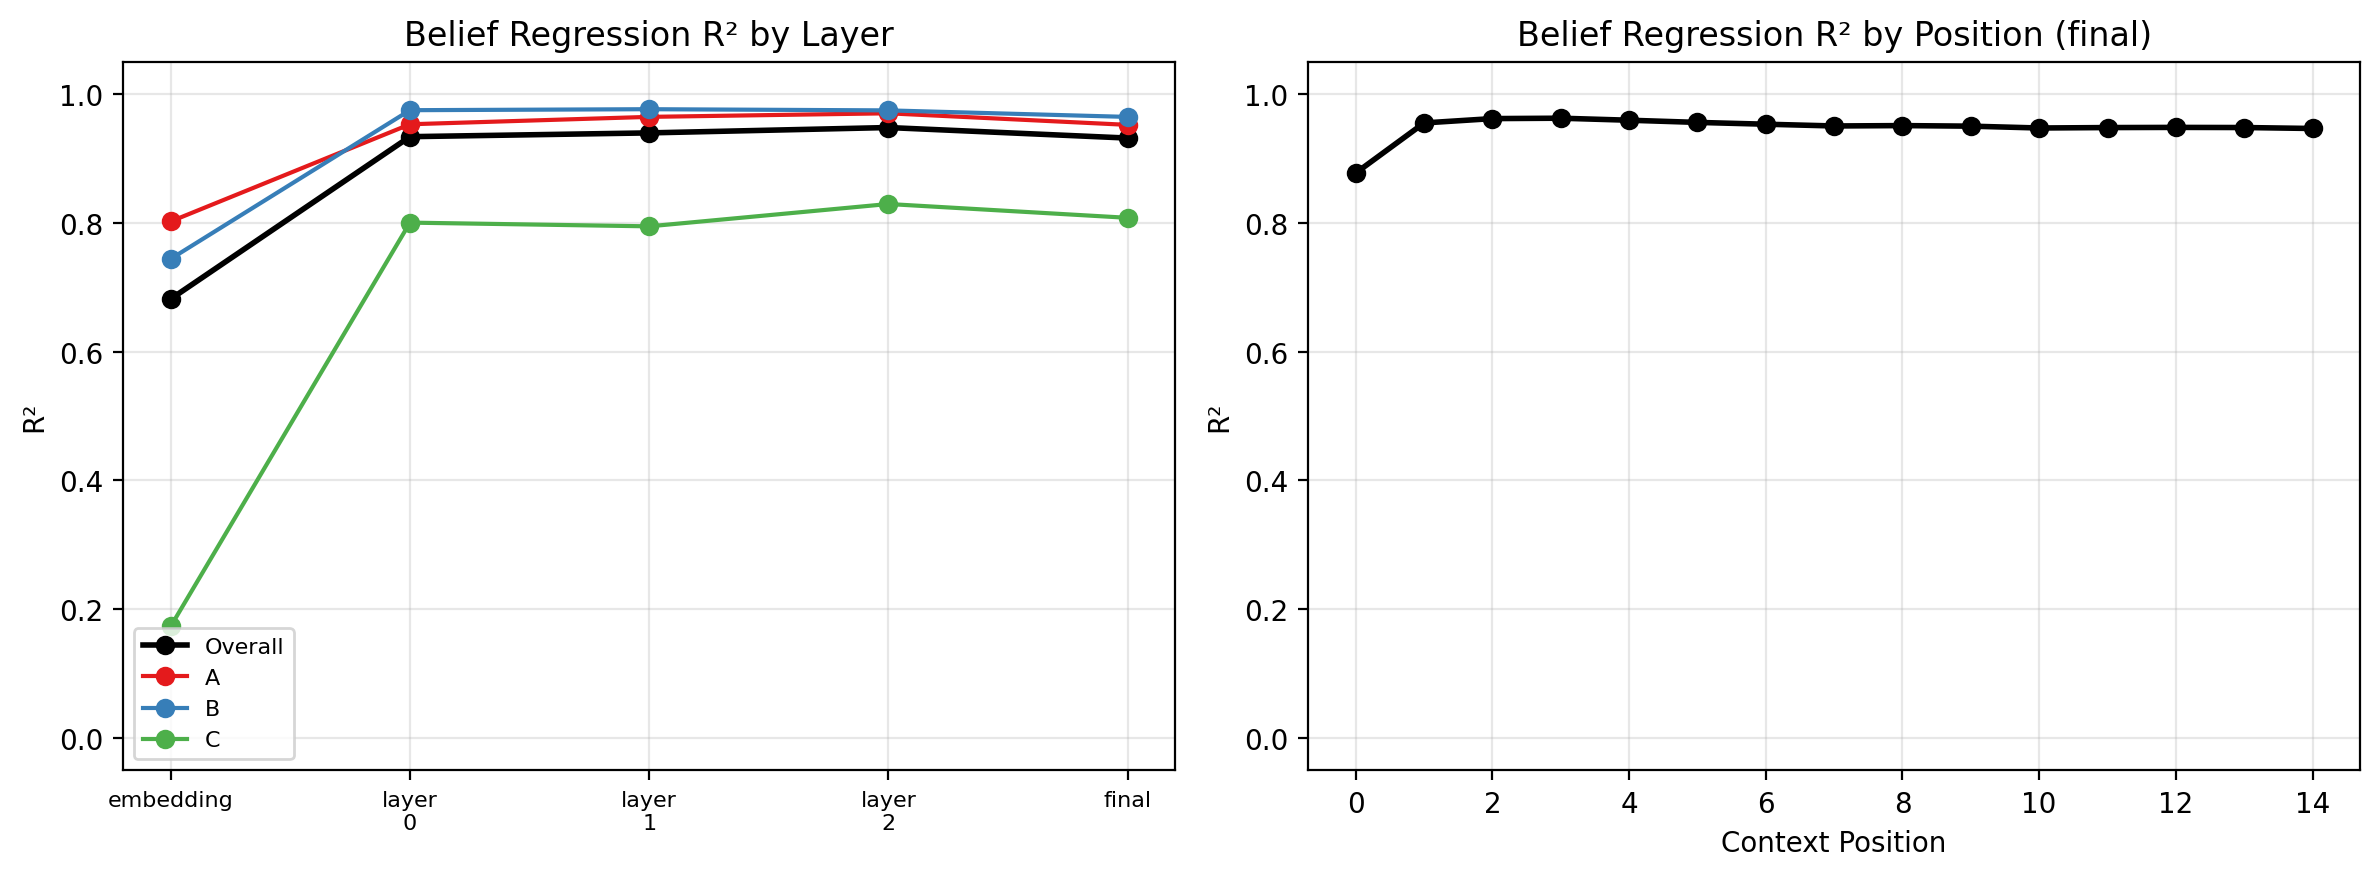
\includegraphics[width=\textwidth]{r2_progression.png}
    \caption{$R^2$ of linear regression from residual stream activations to oracle belief states. Left: by layer, showing that belief information is linearly accessible from the first transformer layer onward. Right: by context position, showing stable encoding throughout the sequence.}
    \label{fig:r2}
\end{figure}

The PCA analysis showed that the top two principal components are dominated by token identity, with no visible component separation. However, the belief information may still be present in the full 64-dimensional residual stream, just not in the directions that PCA prioritises. To test this, we fit linear regressions from the full activation vectors to the oracle Bayesian belief states (\Cref{fig:r2}). $R^2$ jumps from $\sim$0.68 at the embedding layer to $\sim$0.94 at layer 0, then holds steady through to the final layer ($\sim$0.93). Belief geometry is linearly encoded even though it is not visible in a 2D PCA projection. Component C (low $\alpha$, weakly informative tokens) consistently lags behind A and B ($R^2 \approx 0.80$ vs.\ $\sim$0.94--0.97), as expected given that its tokens carry less information about hidden state. Across context positions, $R^2$ rises from $\sim$0.88 at position 0 to $\sim$0.96 by position 2, then remains flat through position 14. The high initial value is not surprising: Mess3 tokens are highly informative, since observing token $k$ strongly implies hidden state $k$ via the emission matrix, so even a single token provides substantial belief information. The jump from position 0 to 2 reflects successful integration of transition dynamics, while the subsequent plateau indicates a stable linear encoding.

\subsection{Recovered Simplices}

\begin{figure}[ht]
    \centering
    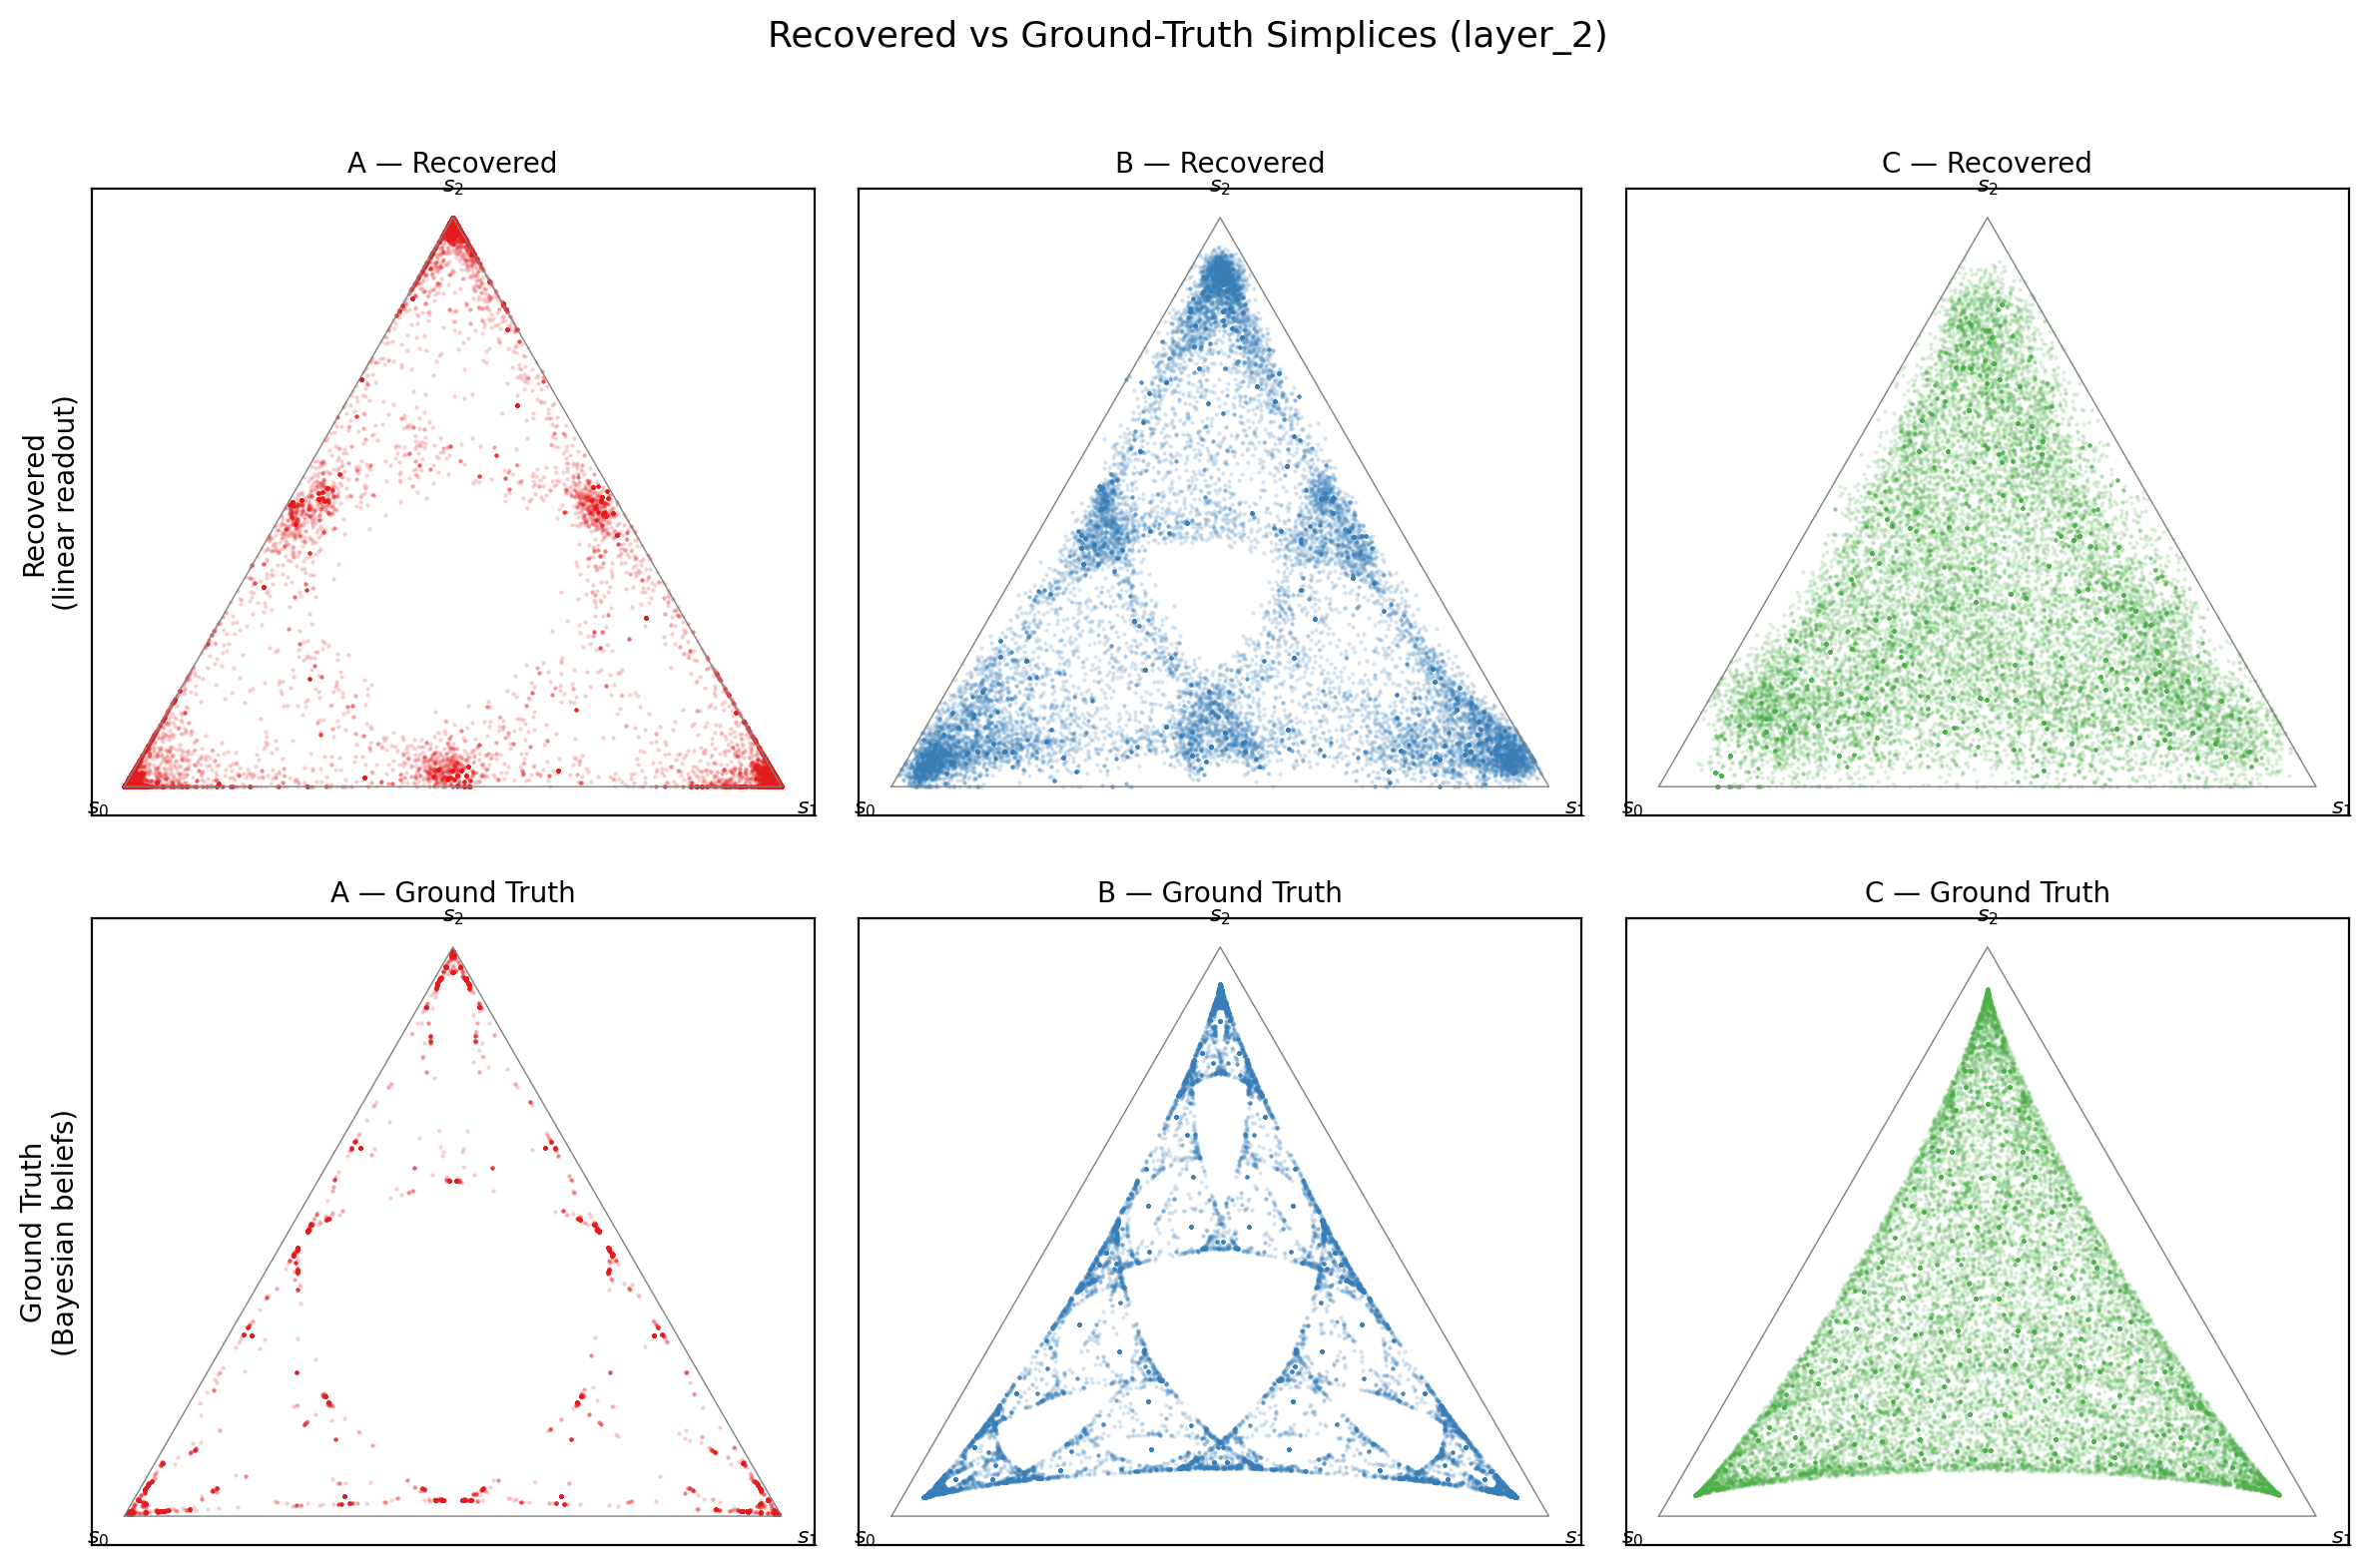
\includegraphics[width=\textwidth]{recovered_simplices.png}
    \caption{Recovered belief simplices from per-component linear regression at layer 2, compared to ground-truth fractal geometry. Top row: linearly decoded from residual stream activations. Bottom row: ground truth.}
    \label{fig:simplices}
\end{figure}

The previous section established that beliefs are linearly encoded in the full residual stream, but used a single global regression: one linear map from the 64D activation vector to the 3D belief vector, fit across all components simultaneously. To test whether the specific fractal geometry predicted in Section 3 is recovered, we instead fit per-component linear regressions at layer 2 (the last transformer block, before the post-LayerNorm representation, which training has shaped to align with the rank-2 unembedding projection and which consequently concentrates into $\sim$2D, obscuring component-specific structure). The distinction matters: if the model encodes each component's beliefs in a different subspace of the residual stream, a single linear map must compromise across these subspaces, while per-component regressions can each find the right one. The per-component $R^2$ values are substantially higher ($>$0.99 for A and B, vs.\ $\sim$0.94 globally), which confirms that the model uses component-specific linear encodings.

The recovered simplices (\Cref{fig:simplices}) closely match the ground-truth Bayesian belief geometry ($R^2 = 0.995$, $0.991$, $0.949$ for A, B, C respectively). Component A shows the predicted sparse, edge-concentrated pattern. Component B shows a triangular structure with a central void, reminiscent of a Sierpinski gasket. Component C shows a dense, filled cloud. This is consistent with the prediction of \citet{shai2024} that fractal belief state geometry is linearly embedded in the residual stream, and shows that it extends to the non-ergodic case where multiple components coexist.

\subsection{Subspace Analysis}

\begin{figure}[ht]
    \centering
    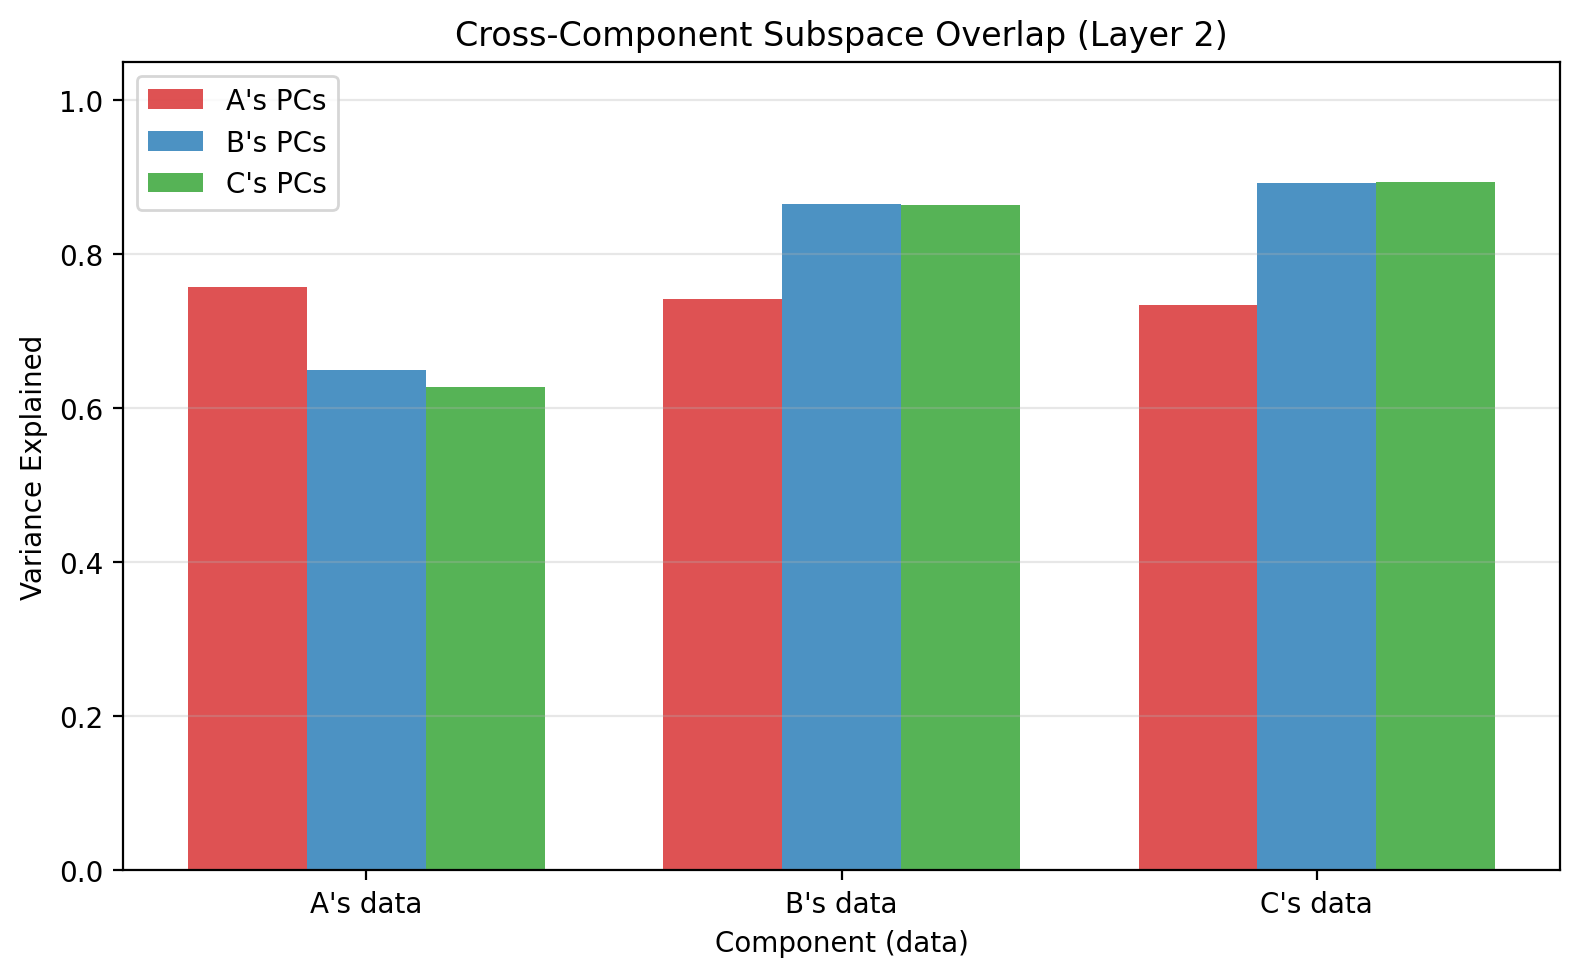
\includegraphics[width=0.7\textwidth]{subspace_cross_variance_layer_2.png}
    \caption{Cross-component subspace overlap at layer 2. Each group shows how much of one component's activation variance is explained by each component's top 3 principal axes. High cross-component values indicate shared subspaces.}
    \label{fig:orthogonality}
\end{figure}

The factored representation hypothesis of \citet{shai2026} predicts that (1) activation dimensionality should scale as $\sum_n (d_n - 1)$ rather than $(\prod_n d_n) - 1$, and (2) the factor subspaces should be mutually orthogonal. These predictions are derived for conditionally independent factors. Our generative model factors as $p(\text{component}) \times p(\text{states, tokens} \mid \text{component})$, but the transition dynamics of the hidden state depend on component parameters $(\alpha, x)$, so within-sequence belief updates are component-specific. The two factors are not conditionally independent given the observations, and the factoring predictions do not strictly apply. Nevertheless, we can examine what structure the transformer learns.

On dimensionality, the effective dimensionality at layer 2 is $\sim$5--6 (from \Cref{fig:explained_variance}), intermediate between the factored prediction of $(3-1) + (3-1) = 4$ and the joint prediction of $(3 \times 3) - 1 = 8$. This suggests partial but not complete factoring.

On subspace structure, we fit PCA separately to each component's activations at layer 2 and measure how much of one component's variance is explained by another component's principal axes (\Cref{fig:orthogonality}). The cross-component explained variance is high, particularly between B and C: each component's top 3 PCs explain nearly as much of the other's variance as its own ($\sim$0.87--0.89 for both self and B$\leftrightarrow$C cross). A's PCs explain less of B and C's data ($\sim$0.73--0.74), and conversely B and C's PCs explain less of A's data ($\sim$0.63--0.65 vs.\ 0.76 self). Component A is thus somewhat more distinct, but the overlap is still substantial. This means the three components share their dominant activation directions. This tests whether different \textit{components} use orthogonal subspaces, not whether the two \textit{factors} (component identity vs.\ hidden state) are orthogonally encoded. Testing the latter would require isolating each factor's contribution, which is complicated by the conditional dependence between our factors.

The shared subspace structure is consistent with the model encoding within-component beliefs in a common set of directions, with component identity represented as an offset. This matches our alternative hypothesis of a shared belief subspace with affine translations rather than orthogonal factor subspaces.

We note a methodological caveat: PCA axes dominated by variance shared across all components will naturally appear in every component's top principal components, so high cross-component overlap may partly reflect this shared-variance artefact rather than genuinely shared representational subspaces. A cleaner test would compute principal angles between component subspaces directly, distinguishing true subspace alignment from trivial overlap induced by shared dominant directions.


\section{Additional Analysis: Component Identification Dynamics}

The previous analyses established that component identity is encoded in the residual stream; we now ask how this encoding develops as the model processes successive tokens. This connects to in-context learning, where a language model must infer the latent mode (topic, domain) from observed tokens.

\subsection{Method} To measure this, we train logistic regression probes on residual stream activations to classify component identity at each (layer, position) pair. As a reference, we compute a Bayesian optimal baseline: the accuracy of an ideal observer who maintains exact posterior beliefs over all 9 joint (component, hidden state) pairs. Comparing probe accuracy to this baseline tells us how close the transformer's linearly-accessible component information is to what is theoretically achievable.

\subsection{Results}

\begin{figure}[ht]
    \centering
    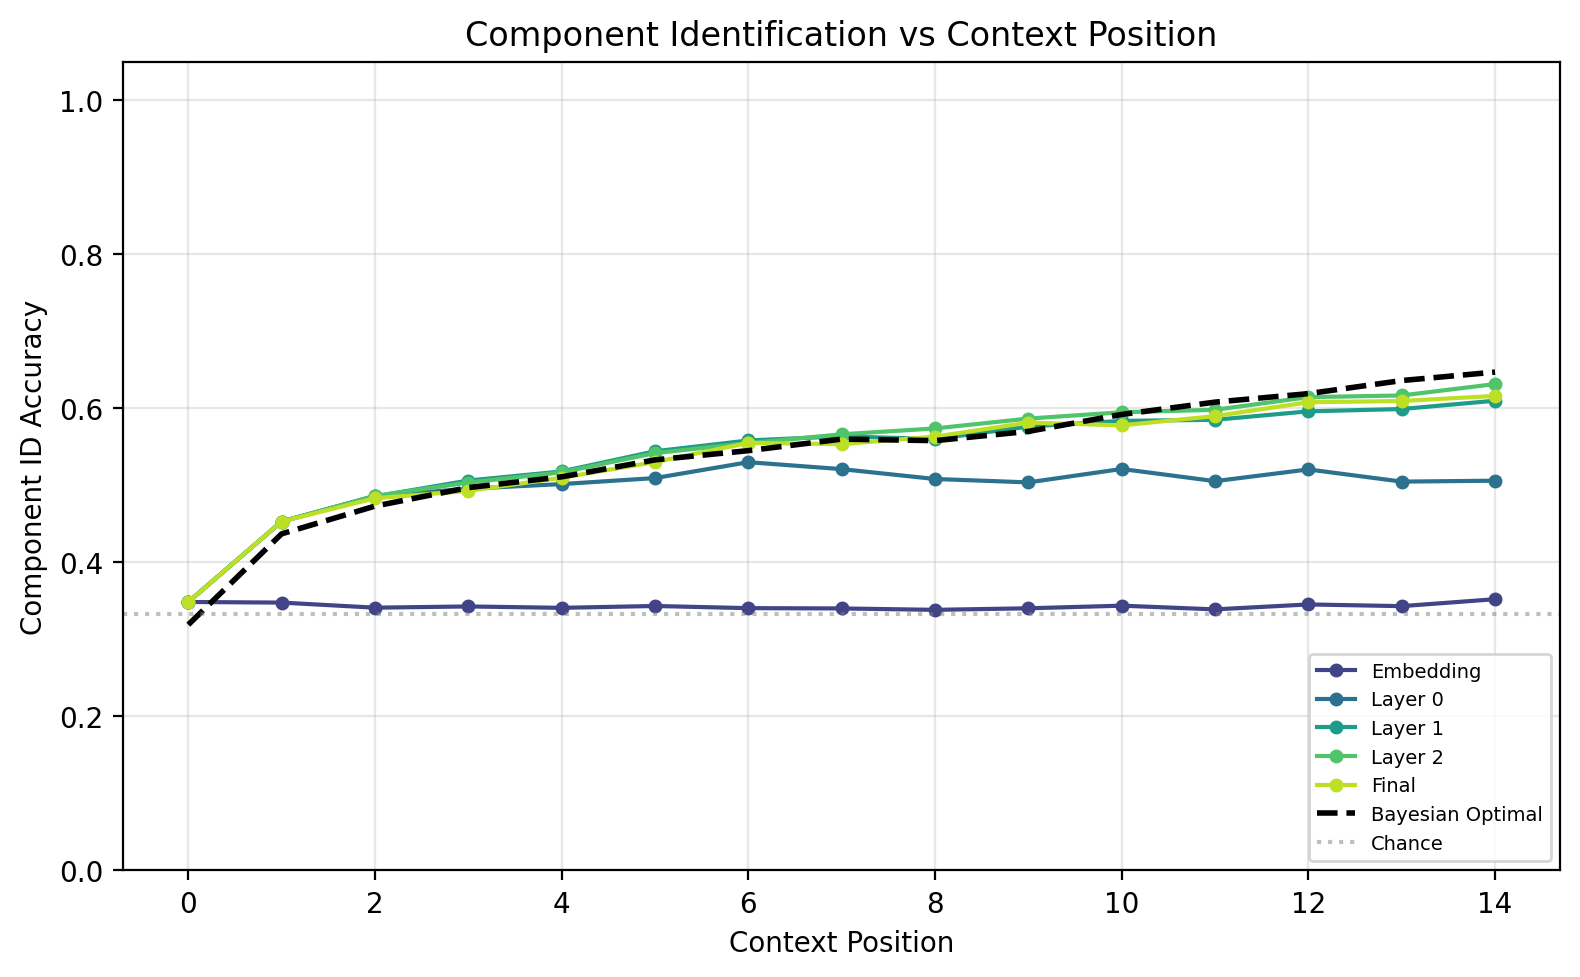
\includegraphics[width=\textwidth]{component_identification.png}
    \caption{Component identification accuracy by context position across layers. Dashed line: Bayesian optimal baseline.}
    \label{fig:component_id}
\end{figure}

The Bayesian optimal baseline (\Cref{fig:component_id}, dashed) rises steadily from chance (33\%) to $\sim$65\% by position 14. The three components' statistics are distinct but require substantial context to reliably distinguish, and even an ideal observer achieves only moderate accuracy with 15 tokens. The embedding layer stays at chance ($\sim$34\%) throughout, so raw token embeddings carry no component information. Layer 0 rises above chance to $\sim$50\% by position 14, as the first attention layer begins aggregating token statistics. Layers 1--2 and the final layer perform best, reaching $\sim$60--63\% at late positions and closely tracking the Bayesian baseline throughout the sequence.

The probe accuracy of $\sim$60--63\% is notable: the model closely approaches the Bayesian optimal baseline ($\sim$65\%), meaning that nearly all theoretically available component information is linearly accessible in the residual stream. The main bottleneck is not the model's representation but the intrinsic difficulty of distinguishing these three components from short sequences: their entropy rates (0.876, 1.387, 1.482 bits) provide limited discriminative signal in 15 tokens.


\section{Discussion}

\subsection{Predictions vs.\ Reality}

Our pre-registered predictions were partially confirmed and partially wrong. What held up: belief states are linearly encoded in the residual stream ($R^2 > 0.9$ from layer 0 onward), per-component fractal geometry is recovered and qualitatively matches ground-truth belief simplices, and component probe accuracy increases with context position and through the transformer blocks. What did not: the final layer compresses to $\sim$2D, far lower than our predicted 4--6D, driven by the rank-2 unembedding head concentrating the representation into the subspace relevant for next-token prediction. Cross-component subspace overlap is high, not low, with shared activation directions rather than the orthogonal factor subspaces we predicted. Component identification reaches $\sim$60--63\%, which is near the Bayesian optimal of $\sim$65\% and thus close to the best achievable accuracy; our prediction of near-perfect separation was wrong not because the model underperforms, but because we overestimated how distinguishable the three components are from 15 tokens. And belief regression $R^2$ is essentially flat across layers and context positions after an initial jump at layer 0, with none of the progressive improvement through layers that we expected.

\subsection{Interpretation}

The $\sim$2D compression at the final layer deserves particular attention. Next-token prediction over 3 tokens requires only a 2-simplex output, and the rank-2 unembedding projection means only a 2D subspace of the post-LayerNorm representation contributes to the loss. Training drives the network to concentrate information there, encoding component identity as location within the 2D prediction simplex and within-component beliefs as fractal structure within each cluster. This matches our alternative hypothesis of a shared belief subspace with affine offsets, rather than the primary prediction of orthogonal factor subspaces. Earlier layers maintain higher-dimensional representations that may be closer to the predicted factored geometry. In effect, the earlier layers maintain a richer encoding that the final layer squeezes down to what the output head needs.

\subsection{Relevance to Language Models}

The model must simultaneously identify which mode generated the sequence, track within-mode belief states, and compress this information into next-token probabilities. It does all three imperfectly. Real language models face the same juggling act, tracking topic and content while producing next-token distributions. Non-ergodicity in natural language operates at multiple timescales: topics and genres at the document level, registers at the paragraph level, syntactic frames at the sentence level. Our Mess3 mixture isolates the simplest case, a single mode drawn once per sequence. The geometric signatures we observe (shared belief subspaces with mode-dependent offsets, compression towards prediction-relevant features at the final layer) may reflect a more general strategy for handling hierarchical non-ergodicity.

\subsection{Limitations}

Our model is small (150k parameters) with short context (15 tokens), which likely limits both component separation and belief tracking. Per-component losses remain 0.09--0.14 nats above theoretical entropy rates, so the model may not have fully converged or may be capacity-limited. Component identification accuracy of $\sim$60--63\% closely approaches the Bayesian optimal ($\sim$65\%), but both are limited by the short context; longer sequences would provide more discriminative evidence between components.


\bibliographystyle{plainnat}
\bibliography{references}



\end{document}
